% !TEX TS-program = pdflatex
%
% Created by Ronald Thisted on 2018-04-24.
% Copyright (c) 2018 .
\documentclass[
  letterpaper, % paper size.
  11pt, % type size.
  % article,
  oneside,  % all pages setup with the same margins.
  % twoside,    % margins change from recto to verso pages.
  onecolumn,  % only one column of text on a page.
  % openright,  % each chapter will start on a recto page.
  % openleft, % each chapter will start on a verso page.
  openany,  % chapters may start on either recto or verso pages.
  article
]{memoir}

\epigraphfontsize{\small\itshape}
\setlength\epigraphwidth{8cm}
\setlength\epigraphrule{0pt}

% Enable hyperlinking/hypertext and PDF metadata
\usepackage{hyperref}

\usepackage[authoryear,round,longnamesfirst]{natbib}
\usepackage{graphicx}
\usepackage{xcolor}
\usepackage{geometry}

\newlength{\parindentsave}

\hypersetup
{
  pdftitle   = {Title},
  pdfauthor  = {Author},
  pdfsubject = {Subject}
}

\title{Reproducing Shakespeare\\{\large In honor of Bradley Efron's 80th Birthday}}
\author{Ronald A. Thisted\\The University of Chicago}

\usepackage{lipsum} % to support fake lorem ipsum text

\begin{document}

\frontmatter

\maketitle

\begin{abstract}
	% Abstract
In 1976, Efron and I published an article studying the problem of estimating the number of unseen species, using as a running example the (unseen) words in Shakespeare's vocabulary that he hadn't employed in the extant corpus of his work.  The approaches we considered required computations that were not then---and are not today---in the repertoire of standard statistical software.  Roughly half way between the appearance of our paper and today, Buckheit and Donoho (1995) introduced ideas of reproducible research.  Here we consider the reproducibility of the figures and tables in the Shakespeare paper, what we might have done in 1976 that would have aided reproducibility in 2018, and what lessons that exercise suggests for maximizing the likelihood that today's computationally intensive research can be reproduced in decades to come.

\end{abstract}
\clearpage

\tableofcontents*
\clearpage

\mainmatter

\chapter[Introductory Matter]{Introduction}
\epigraphfontsize{\small\itshape}
% epigraph
\epigraph{
	So on the tip of his subduing tongue\\
	All kind of arguments and question deep,\\
	All replication prompt and strong,\\
	For his advantage still did wake and sleep.}
{--- \textit{A Lover's Complaint}} %120--123

	In 1976, Efron and I published a paper in \textit{Biometrika} that explored aspects of the unseen species problem, \textit{i.e.,} how to estimate the number of unseen types based on the distribution of counts of types that had been observed \citep{Efron:1976zs}, henceforth ET.  The motivating---and captivating---example we used was to estimate the number of words that Shakespeare knew but which he had never been seen to use in his published corpus of plays and poetry.  The paper generated considerable interest at the time, and a follow-on paper some ten years later concerning potential Shakespearean authorship of a (not very good) poem that had recently been discovered led to a minor industry in developing quantitative methods to judge matters of Shakespearean authorship.  Originally viewed as frivolous by serious scholars of Shakespeare, ``stylometrics'' has come to have a recognized place in literary debate. [Mention \textit{Federalist}, Elliott/Valenza, Foster].
	
	In the ensuing years, interest in our original paper has been unabated, and it has continued to be cited---some 478 times as of May 2018 according to Google Scholar.  Over the years a number of readers have contacted one or the other of us to suggest what we should have done, or to inform us of the logical flaws in our analysis, or most commontly, to ask questions about what we did or how we did it.  We tried to respond to simple queries as best we could, and where we could not each of us would suggest to our correspondents that they contact the other.
	
	Last year Brad received a query from a Chinese student who sought to understand how we got some of the results we reported in the 1976 paper, and Brad suggested that the student write to me.  The main query was how we obtained the parameter estimates for the negative binomial model that we reported in Table~3.  Surely, I thought, I could whip together a few lines of code that I could send to our correspondent to help him on his way.  I soon discovered that it wasn't any longer quite obvious just what that negative binomial model consisted of---that is, the likelihood to maximize wasn't immediately obvious, even from reading our pellucid article.  It also wasn't a straightforward task to get maximum likelihood estimates from any of the plausible candidate models.  And there was a cryptic comment in the manuscript whose import also wasn't immediately apparent: ``Table~3 shows the maximum likelihood fits, obtained by iterative search for various choices of $x_0$.''
	
	The challenge of reproducing a key ingredient of our 1976 paper evokes the current focus on ``reproducible research,'' a concept introduced to the statistics community by Buckheit and Donoho in their influential \citeyear{Buckheit:1995hl} paper, which is related to Donald Knuth's notion of ``literate programming'' \citep{knuth1984literate}, and one for which I and many others have advocated as a fundamental building block for quality science.  Had Brad and I created a reproducible manuscript when we were writing our paper, in 2018 we would have the benefit of our 1976 selves both telling us and showing us exactly what they had done.
	
	It seemed like a fitting project to explore the answers to two questions: (1) what would a reproducible manuscript for the Shakespearean vocabulary paper look like today, and (2) what challenges might thwart achieving a result that would still be useful some $40+$ years after the original writing.
	
\chapter[Elements of reproducibility]{Elements of reproducibility}

	In this project, we take ``reproducibility'' to mean the ability to reproduce, from the original data, the main computations, tables, and figures from a report of research work.  Ideally, a compendium of the artifacts that enable a work to be reproduced, along with the work itself, will be available to the scientific community to check, to modify, and to build upon.
	
There are (at least) four components of a research project compendium that affect the ability for the final article to be reproduced:
	\begin{enumerate}
		\item the computer programs or scripts used for calculation,
		\item the underlying data,
		\item the hardware and operating system under which those programs were run, and
		\item the choices of inputs to the calculations, and the process by which those choices were made.
	\end{enumerate}
	
	  In our case we shall focus on a subset of the main calculations and figures from \citet{Efron:1976zs}. In the Shakespeare case, we are up against some challenges in each of these domains listed above, however in this talk we shall focus primarily on the first of these factors, with a few words reserved for the other three items.  Specifically, we shall take as given the raw data reported in ET, and then undertake to reproduce calculations in the paper conditional on the reported data.
	  
	  The data, programs, and results of this investigation are available from a GitHub repository (\texttt{https://github.com/rthisted/EfronAt80}), from which they can be freely accessed.
	
\section{Computer programs} % (fold)
\label{sec:computer_programs}

One of the key ideas of reproducible research is that it is a means to communicate not only with colleagues who may wish to understand or to build on our work, but also to communicate with our future selves when we seek to remind ourselves of what we did and how we did it.  Since there is no GitHub repository of the work we did---GitHub not having been invented until 33 years after we started our work---I had to rely on the next best thing, namely, paper files from that era.  Those files are part of my papers that have undergone many moves and many downsizings; it wasn't obvious to me that I would have kept anything of value.  But as it turns out, at least some useful material survived, a testament to the enduring value of paper records, a storage medium and communications format that has survived the test of time.
  
The ET paper relies heavily on computations based on the raw data in Table~1 of ET, reproduced in Figure~\ref{fig:ETT1}, for which custom programs were written, together with some calculations that were apparently done ``by hand'' using the calculator technology of the day.

The main computations appear in Tables~2 through~7.  Table~3 shows maximum likelihood parameter estimates for Fisher's (truncated) negative binomial model for various choices of the truncation parameter, and Table~2 shows the estimated means for word types seen exactly $x$ times calculated from one set of the negative binomial parameters.  Table~4 shows calculated Euler coefficients for the generalized linear vocabulary estimator.  Table~5 contains calculated lower bounds for the expected number of new words that one would see in a body of work $t$ times as large as Shakespeare's extant corpus, and Table~6 shows lower and upper bounds for the same quantities based on a linear programming formulation of the problem.

\begin{figure}
	\centering
	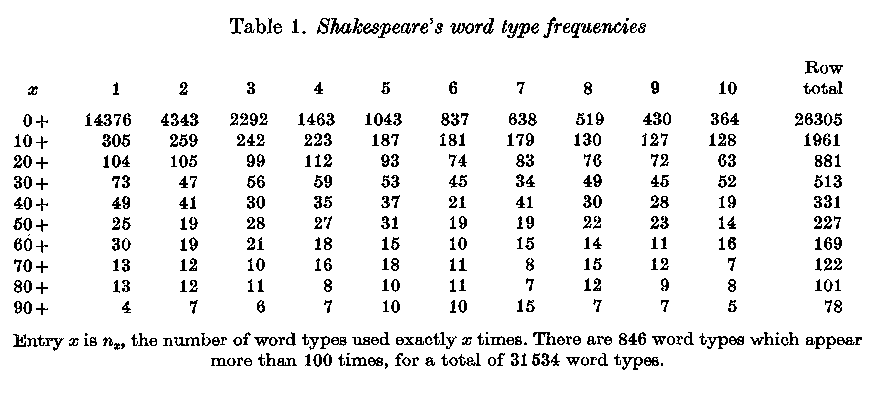
\includegraphics[width=5in]{../compendium/Figures/ET-Table1.pdf}
	\caption{Table~1 from Efron and Thisted \citeyear{Efron:1976zs} }
	\label{fig:ETT1}
\end{figure}

\subsection{Computing circa 1975} % (fold)
\label{sub:computing_circa_1975}
The first task is to determine whether we can replicate the main results, here taken to be the contents of Table~3 from Efron and Thisted \citeyear{Efron:1976zs}\footnote{In this paper we shall focus on the calculations in Tables~2 and~3 to illustrate the issues involved; the calculations of Tables~4 through~6 raise additional difficulties which are beyond the scope of this project; we touch on those issues briefly.}.  These target results are displayed in Figure~\ref{fig:ETT3}

\begin{figure}
	\centering
	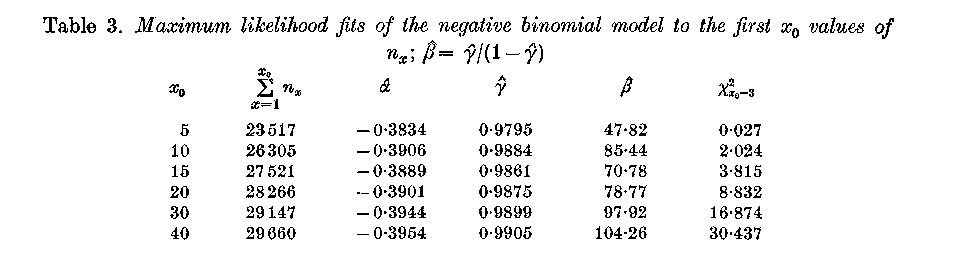
\includegraphics[width=6in]{../compendium/Figures/ET-Table3.pdf}
	\caption{Table~3 from Efron and Thisted \citeyear{Efron:1976zs}.  These are the main results whose reproducibility is at issue. }
	\label{fig:ETT3}
\end{figure}

A starting point is what we did in 1975 when working on our paper.

The computer programs for those calculations used the technology of the day, which in this case involved writing programs in a dialect of BASIC, PL/I, and a script for a IBM proprietary mathematical programming system called MPS/360. As near as I can reconstruct, the PL/I programs were used to generate the input to the MPS software, which was used to solve a large linear optimization program.  IBM discontinued sales and support of MPS in 2005. At the time \texttt{S}, (the statistical programming language that John Chambers developed at Bell Laboratories and the predecessor to \texttt{R}, did not yet exist.  Indeed, there were no general-purposed statistical programming environments on which to draw.

Fortunately, one of us (Thisted) not only seems to have saved large chunks of the working papers from the Shakespeare project, but also to have refrained from tossing them out in the course of multiple relocations and office downsizings.  And I was able to find what may be a program that was used to perform the calculations in Table~3. This program is shown in Figure~\ref{fig:mle-bas-orig}.

\begin{figure}
	\centering
	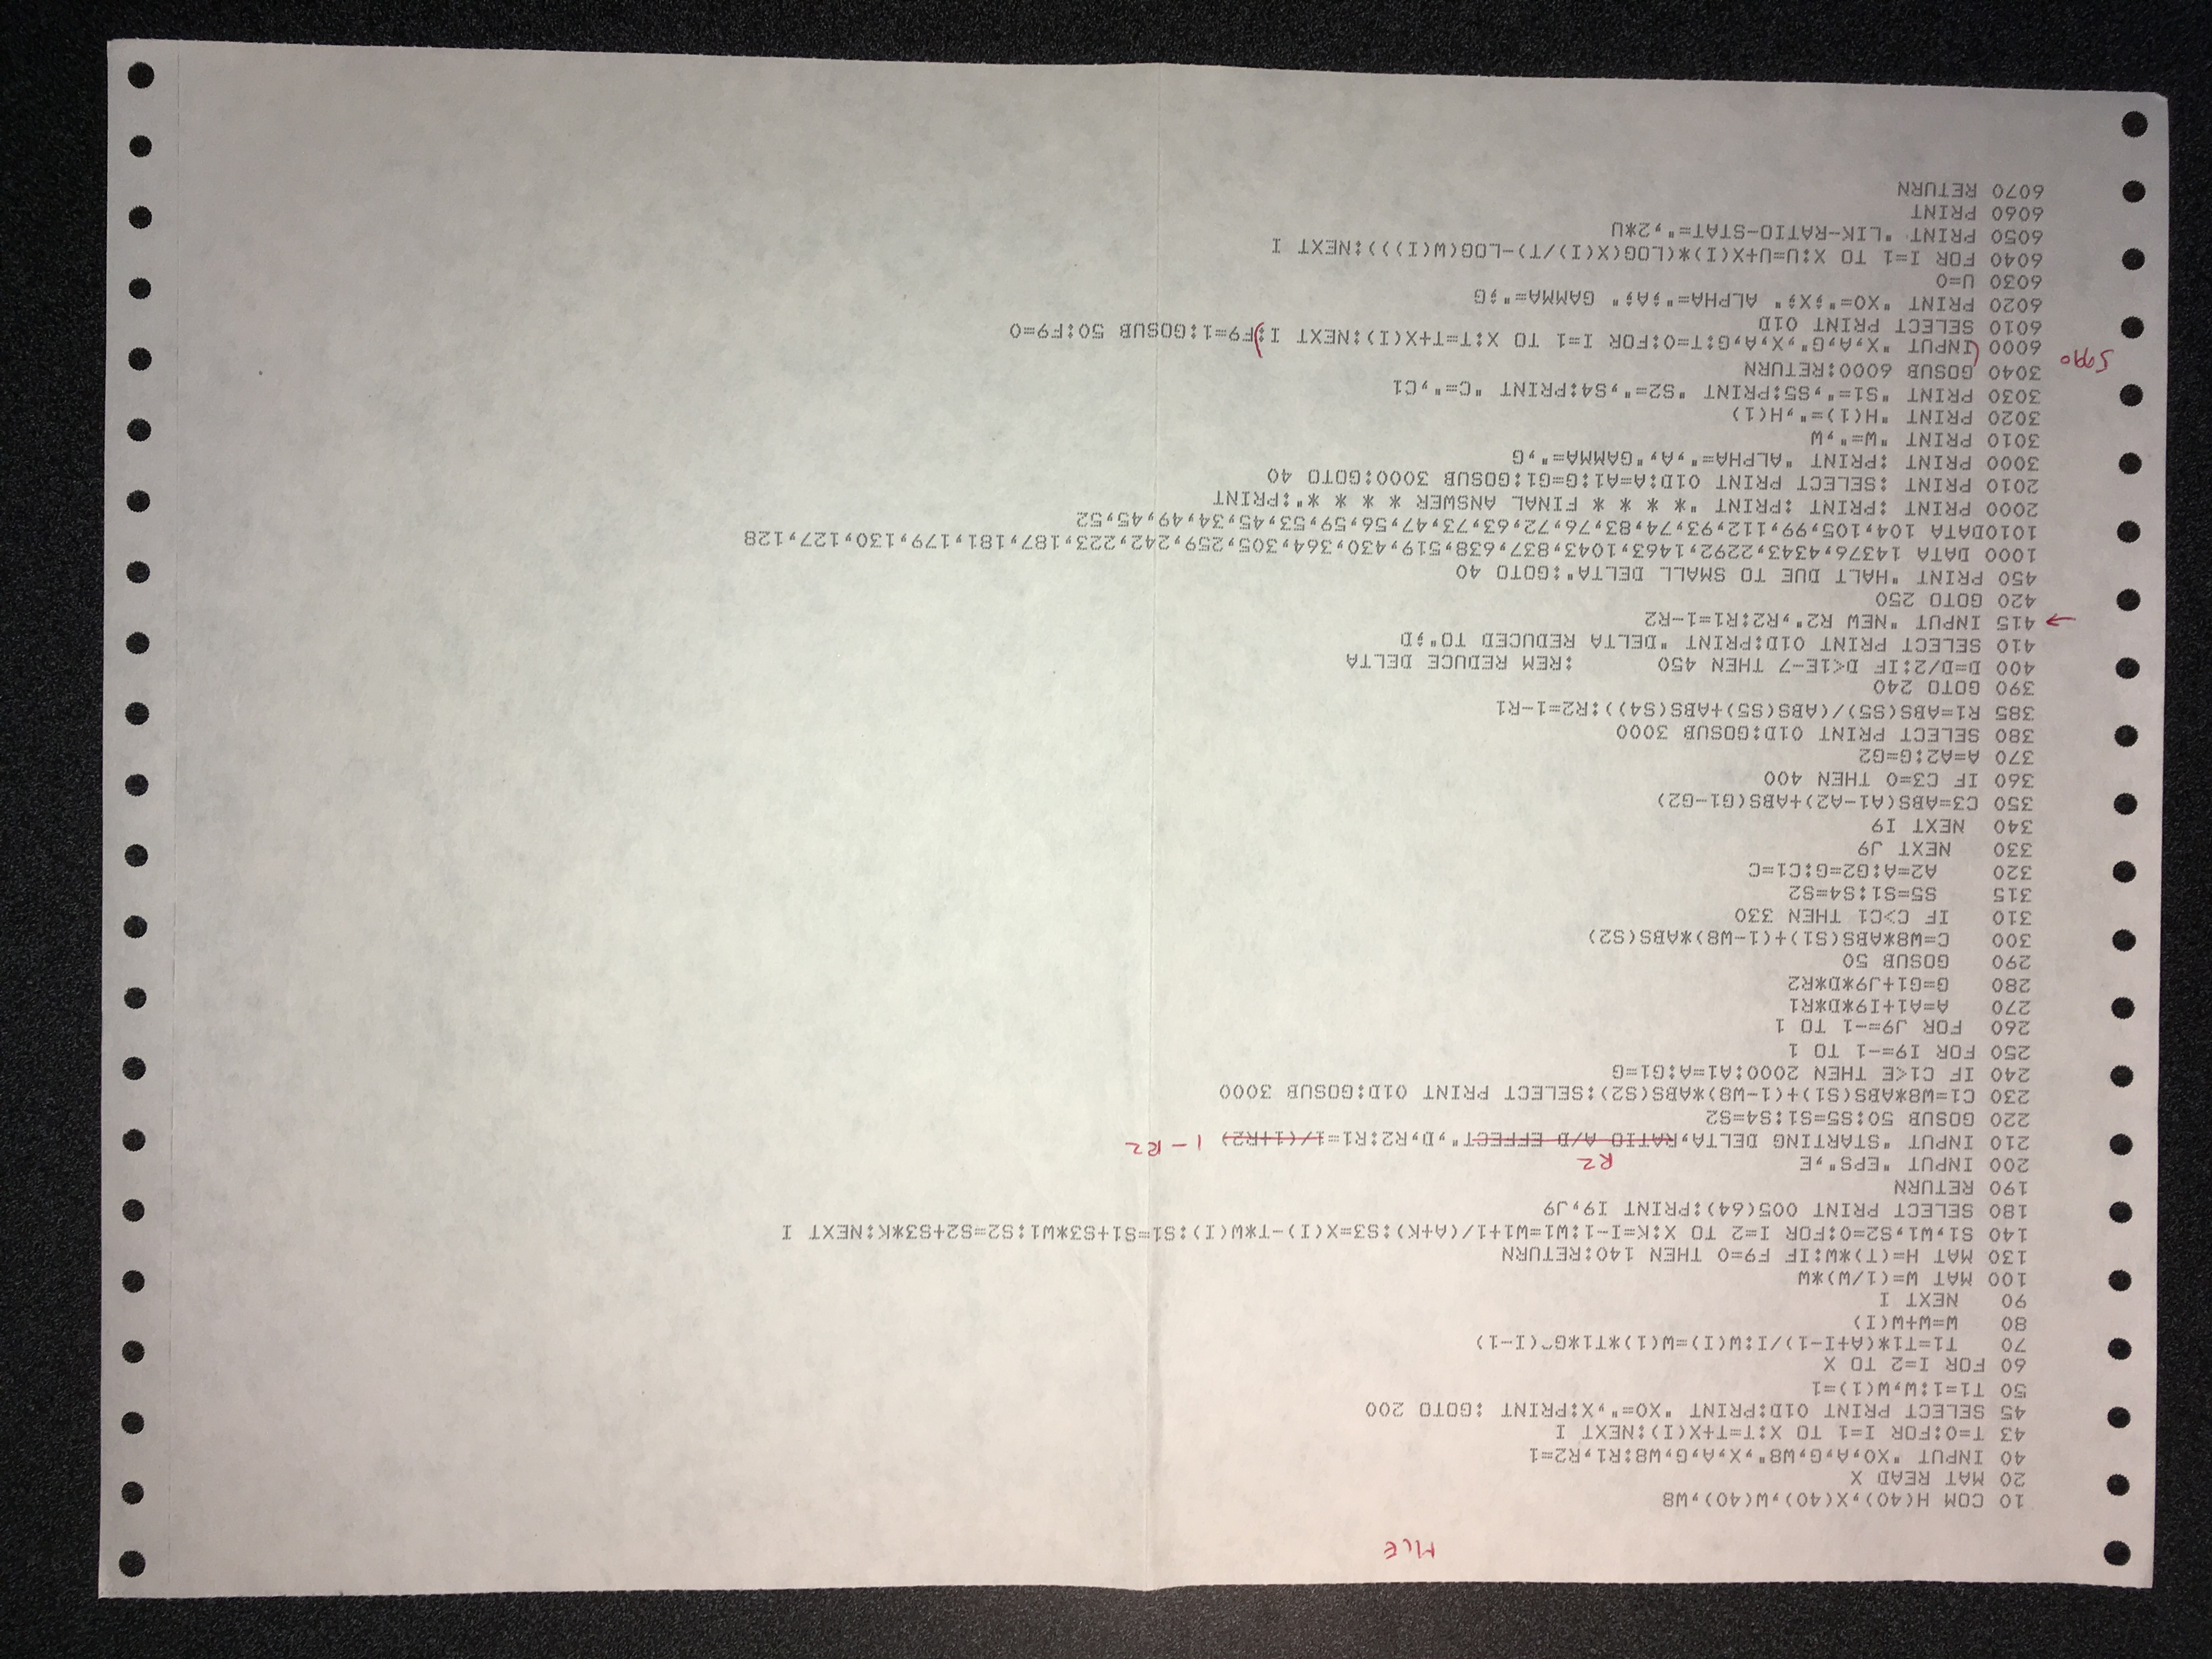
\includegraphics[width=5in,angle=180]{Photos/mle-bas-5036.jpg}
	\caption{Program used to calculate maximum likelihood estimates in Table~3 of Efron and Thisted \citeyear{Efron:1976zs} }
	\label{fig:mle-bas-orig}
\end{figure}

This program was written for the Wang~2200 computer, the departmental computing device of the time, which could be only programmed in this dialect of BASIC.  The program was transcribed, and is included both in Appendix~\ref{cha:basic_mle_program} and in the GitHub repository \texttt{compendium/Programs/mle.bas.txt}.  Unfortunately, there are no Wang~2200s available to me on which I can run this program which, I note, requires manual input of starting values and convergence parameters.

The inputs and outputs to this program were not, unfortunately, among the pieces of papers that I preserved, although one page, shown in Figure~\ref{fig:Table3-output-5037a}, gives a hint, both as to where one set of values (corresponding to $x_0=40$) may have come from, and to how much the process of what actually transpired has been lost.  It is also clear that the output in this figure was not produced by the computer program in Figure~\ref{fig:mle-bas-orig}.  It isn't clear whether the preserved output is from an early prototype of the final program, or the preserved program is an early prototype of the one that produced the output of the latter.

\begin{figure}
	\centering
	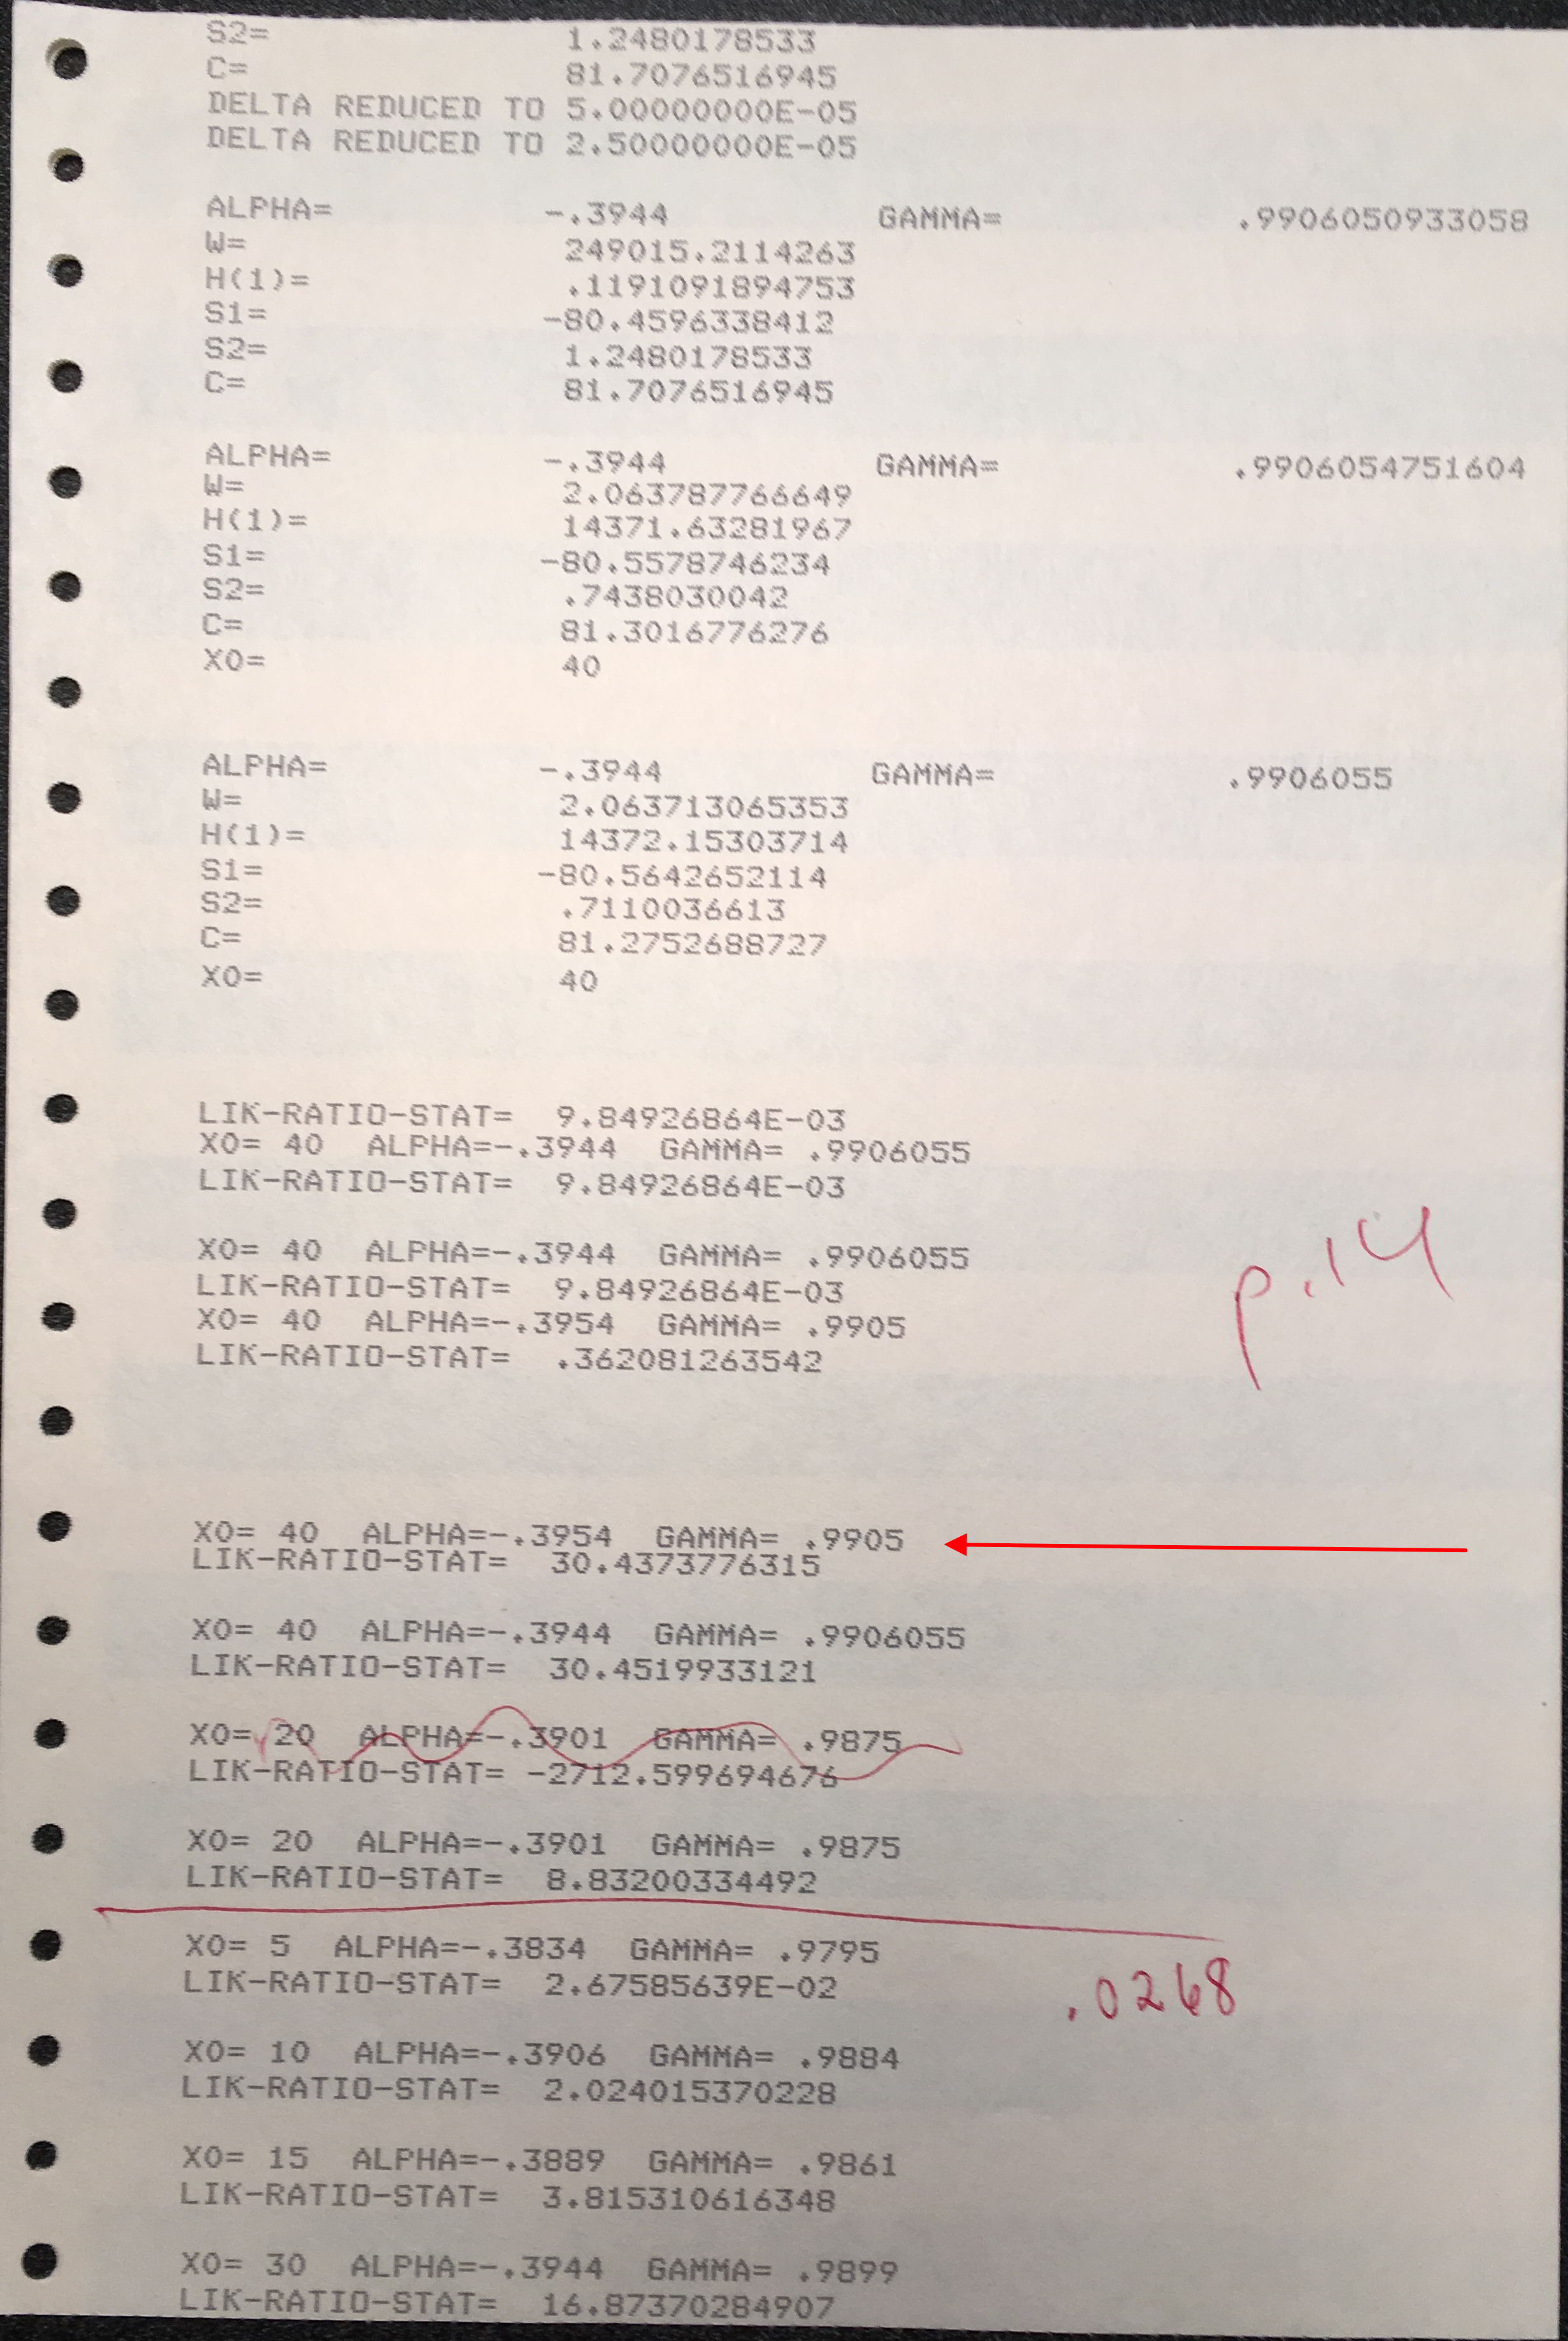
\includegraphics[width=3in]{Photos/Table3-output-5037a.jpg}
	\caption{The apparent source for $\hat\alpha$ and $\hat\gamma$ corresponding to $x_0=40$ in Table~3 of Efron and Thisted \citeyear{Efron:1976zs}.  The red arrow points to the parameter values that appear in the published table. }
	\label{fig:Table3-output-5037a}
\end{figure}

% subsection computing_circa_1975 (end)

\subsection{Recomputing Table~3 from Table~1} % (fold)
\label{sub:recomputing_table_3_from_table_1}

	So how would we do this computation in 2018, and do so in a way that might be more readily reproduced 40~years hence than our work from 40~years ago seems to have been?  The first step is to determine just what model is being fit.  Although the paper itself isn't crystal clear on the point, the model corresponding to $x_0$ is simply fitting a multinomial with $x_0$ categories (corresponding to $x=1$ through $x_0$), the probability $p_x$ for category $x$ being proportional to
$$
p_x \propto {\Gamma(x+\alpha) \over x! \Gamma(1+\alpha)}\gamma^{x-1},
$$
for $\gamma<1$ and $\alpha>-1$, and where $n_x$ is the number of word types observed in category $x$.  The trickiness in the calculation results from the ``proportional to'' description of the probabilities, as the proportionality factor that ensures the probabilities sum to unity itself is a function of the parameters. 
	
	In response to one of the recent queries about how we got the values in Table~3, I resorted to the quickest (and dirtiest) method possible: I used the black-box optimizer built into Excel!  This spreadsheet (\texttt{ET-Table3-origdata.xlsx}, locked 12:36pm CDT 12 May 2018) is available in the GitHub repository for those interested.  This required building a separate pane for each choice of $x_0$, in which the calculations were performed.  The results analogous to ET's Table~3 are in the Summary pane, and are reproduced in Table~\ref{tab:excel}.
	
\begin{table}
	\centering
	\begin{tabular}{rrrrrr}
$x_0$ & $\sum n_x$ & $\hat\alpha$ & $\hat\gamma$ & $\hat\beta$ & $\chi_{x_0-3}^2$\\[3mm]
 5  & 23517  & -0.3834 &  0.9795 &   47.71 &   0.027\\
10  & 26305  & -0.3902 &  0.9883 &   84.48 &   2.024\\
15  & 27521  & -0.3867 &  0.9854 &   67.42 &   3.752\\
20  & 28266  & -0.3894 &  0.9872 &   77.20 &   8.822\\
30  & 29147  & -0.3945 &  0.9899 &   98.18 &  16.873\\
40  & 29660  & -0.3973 &  0.9912 &  112.22 &  30.437\\
\end{tabular}


	\caption{Maximum likelihood estimates calculated using Microsoft Excel's built-in optimizing routine.}\label{tab:excel}
\end{table}

	A comparison of Table~3 from ET shown in Figure~\ref{fig:ETT3} and the results from Excel in Table~\ref{tab:excel} shows reasonably good agreement, although there are a few things to note.  First, the results for $\hat\alpha$ agree in the first two decimal places, but diverge in the third, with the greatest divergence for $x_0=40$.  Second, the $\chi^2$ values for the Excel calculation are always less than or equal to those of the original calculation.  This suggests that Excel is actually finding a slightly larger value for the maximized log likelihood.  Third, although the $\chi^2$ values are identical at $x_0=40$, the values for both $\hat\alpha$ and $\hat\gamma$ differ in the third decimal place, which suggests that the likelihood function is relatively flat in the neighborhood of the solution.
	
	Of course if the goal is to maximize reproducibility in the future, an Excel spreadsheet is very nearly the worst possible choice.  Such spreadsheets are easily corrupted by accident, provide no method for documenting changes, and are opaque as to computing formul\ae\ and processes.

	Today there are many well-supported programming environments with high-quality numerics and descriptive scripting languages that make even  non-standard problems like that of fitting the Fisher negative binomial model relatively straightforward to solve.  For purposes of recreating Table~3, I used Stata \citeyear{StataCorp:2017aa}, a computer package widely used by epidemiologists, biostatisticians, and econometricians, since it has a general-purpose maximum likelihood capability.  Stata also has a strong focus on both the quality of the numerical algorithms it employs and on documentation of those algorithms, so using Stata affords a comparison with the black-box, unscripted Excel spreadsheet.
	
	Solving the problem in Stata involves two scripts.  The first contains a program that calculates log-likelihood values that Stata's built in maximum likelihood program (\texttt{ml}) calls when it is run; the second is the wrapper for the calculation that invokes the \texttt{ml} command as applied to the model at hand.  These scripts are reproduced in Appendices~\ref{cha:stata_negative_binomial_log_likelihood} and~\ref{cha:stata_table_3_reproduction} (as well as the GitHub repository at \texttt{compendium/Analysis/et.do} and \texttt{compendium/Analysis/table3mlFromTable1.do}, respectively.)  Both scripts include the line ``\texttt{version 15.1}'', which ensures that should the script be run under later versions of Stata, it will be executed under the rules prevailing under version~15.1.
	
	The results from running the Stata script are given in Table~\ref{table:Stata}, which also includes a line for $x_0=100$, a set of values that we did not calculate in~1975.
	
\begin{table}
	\centering
	\input{StataMLE-Table3-origdata}
	\caption{Maximum likelihood estimates calculated using Stata's \texttt{ml} program for maximum likelihood calculation, coupled with the user-written likelihood specification script \texttt{et.do}.}\label{table:Stata}
\end{table}
	
	The Stata-based results agree very well with those from the Excel spreadsheet, with values for $\hat\gamma$ being identical between the two, and values for $\hat\alpha$ differing by no more than one unit in the fourth decimal place.  Stata also provides asymptotic standard errors for the parameters.

% subsection recomputing_table_3_from_table_1 (end)

% section computer_programs (end)

% Data

\section{Data sources} % (fold)
\label{sec:data_sources}

One posssible reason for non-reproducibility is using a data set for the reproduction enterprise that is actually different from the data set used in the original investigation.  The inability to reproduce the estimate of $\hat\Delta(1)=11430$ from equation~(2.5) by applying expression~(2.4) to the data in Table~1 suggests that this might be the case.

The data on which the paper is based consist of the counts of the number of ``word types\footnote{A ``word type'' is a lexicographically distinct string of characters.  Plural versions of singular nouns constitute distinct word types, as do different tenses of the same verb.  Different meanings of the same word, e.g., ``bear'' as a verb and as a noun are not distinguished; they are the same word type.}'' $n_x$ that appear in the Riverside edition of Shakespeare's complete works exactly $x$ times.  For instance, there are 14375 word types that appear on only one occasion in Shakespeare, and there are 4343 word types that appear on exactly two occasions.  These word type frequencies are displayed in Table~1 of ET for the 30688 word types that appear 100 times or fewer.  An additional 846 word types are said to appear more than 100 times each, but their exact frequencies are not supplied in the ET article.

The counts in Table~1 were taken from secondary sources, and reproducibility of the results would be enhanced if we could confirm at this remove that, for instance, there were no transcription errors in extracting data from the original sources.

The sources for these frequencies are ``based on Spevack's \citeyearpar{Spevack:1968qd} concordance and on the summary appearing in an unpublished report by J.~Gani and I.~Saunders.''  An article apparently based on the report appeared in the 1976 volume of \textit{Sankhy\=a} \citep{Gani:1976rg}.  That article contains a table that exactly reproduces the first two lines of ET's Table~1, which suggests that both ET and \citeauthor{Gani:1976rg} were both based on a common original source.  Because \cite{Gani:1976rg} does not contain the counts for $x=21$ through $100$, we surmise that either those values were contained in the unpublished technical report referred to in ET but omitted for space reasons in the published version, or that there is a third source based on \citeauthor{Spevack:1968qd} that contains those values.

Fortunately, Spevack's six-volume \textit{Concordance} resides in the University of Chicago's Regenstein Library, which I consulted in the hopes that these questions could be resolved.

\subsection{High frequency counts} % (fold)
\label{sub:high_frequency_counts}

Appendix~A in volume~6 of \citeauthor{Spevack:1968qd} lists all of the words in the Shakespearean corpus by frequency.  Starting with the most frequently used words, the word ``the'' appears 27457.  Because there is only one such word with that frequency, $x_{27457}=1$\footnote{As explained in section~\ref{sub:double_counting}, $x_{27457}$ should probably be taken to be zero, as the frequency count for ``the'' should be greater than 27457.}.  Each observed frequency is listed, followed by a list of all of the words having that frequency.  The first page of Spevack's Appendix~A, together with a more typical page, are shown in Figure~\ref{fig:appendixa}.

\begin{figure}
	\centering
	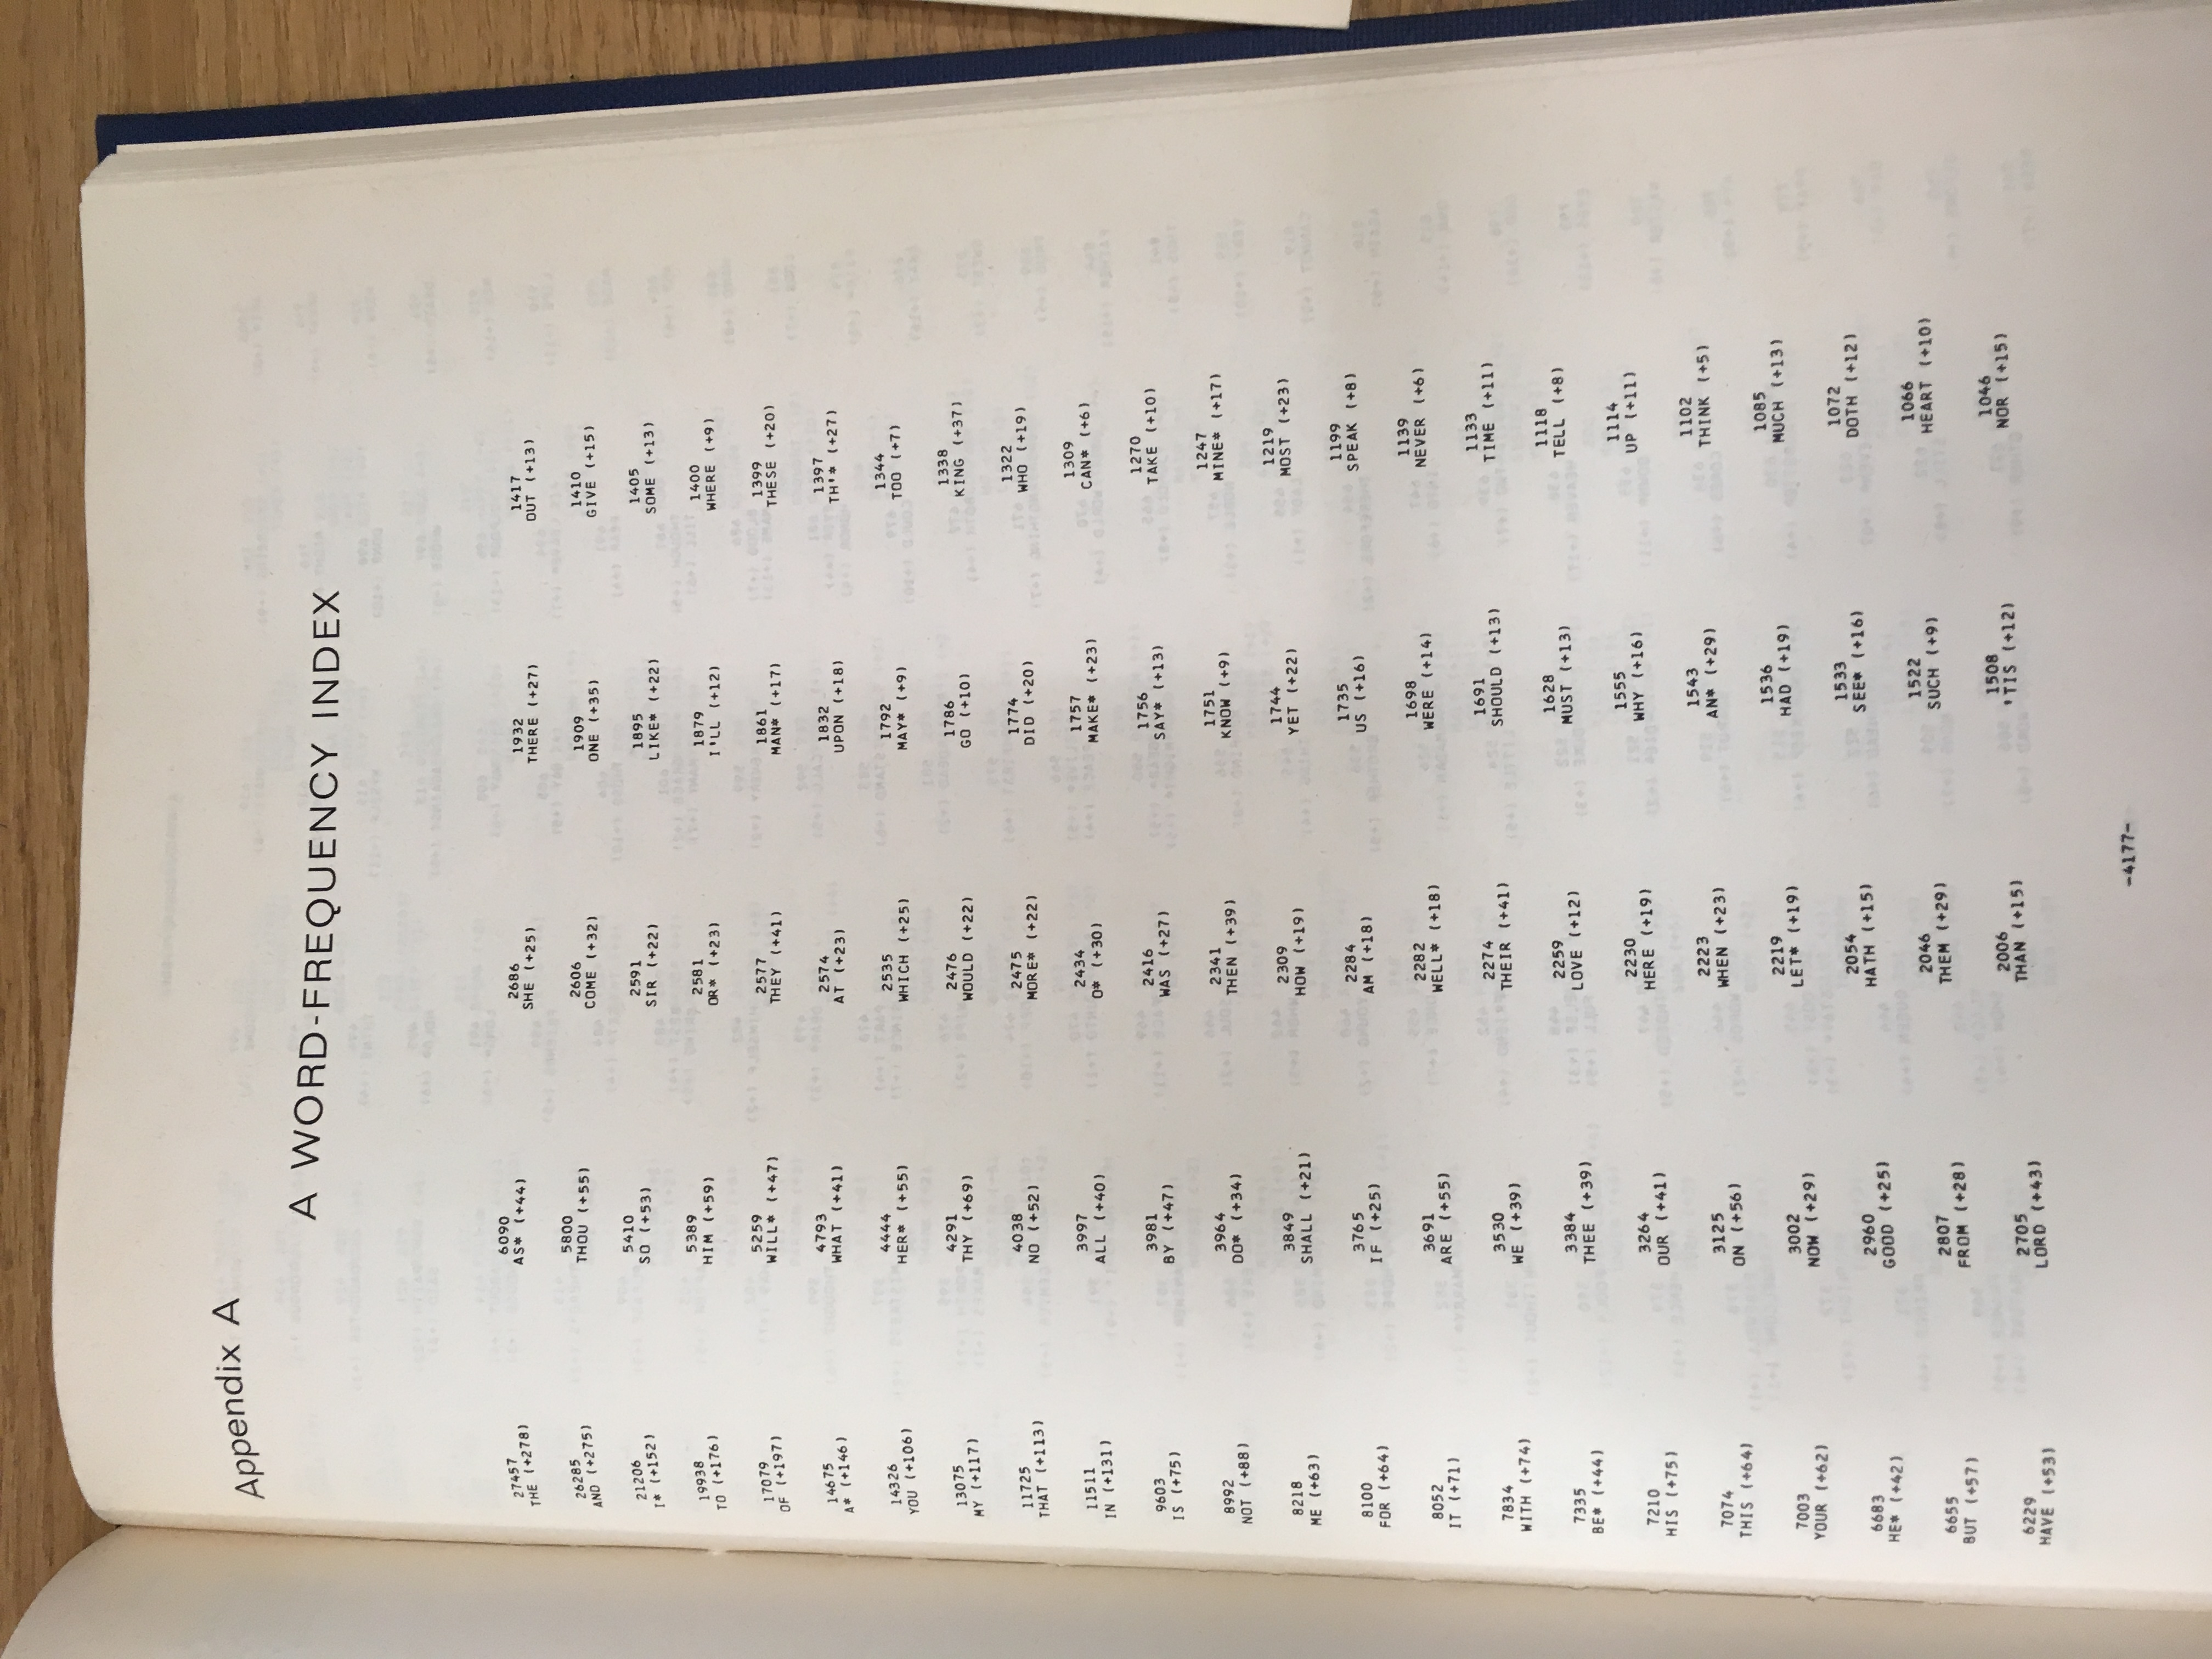
\includegraphics[width=3.25in,angle=270]{../compendium/Figures/IMG_4943.jpg}
	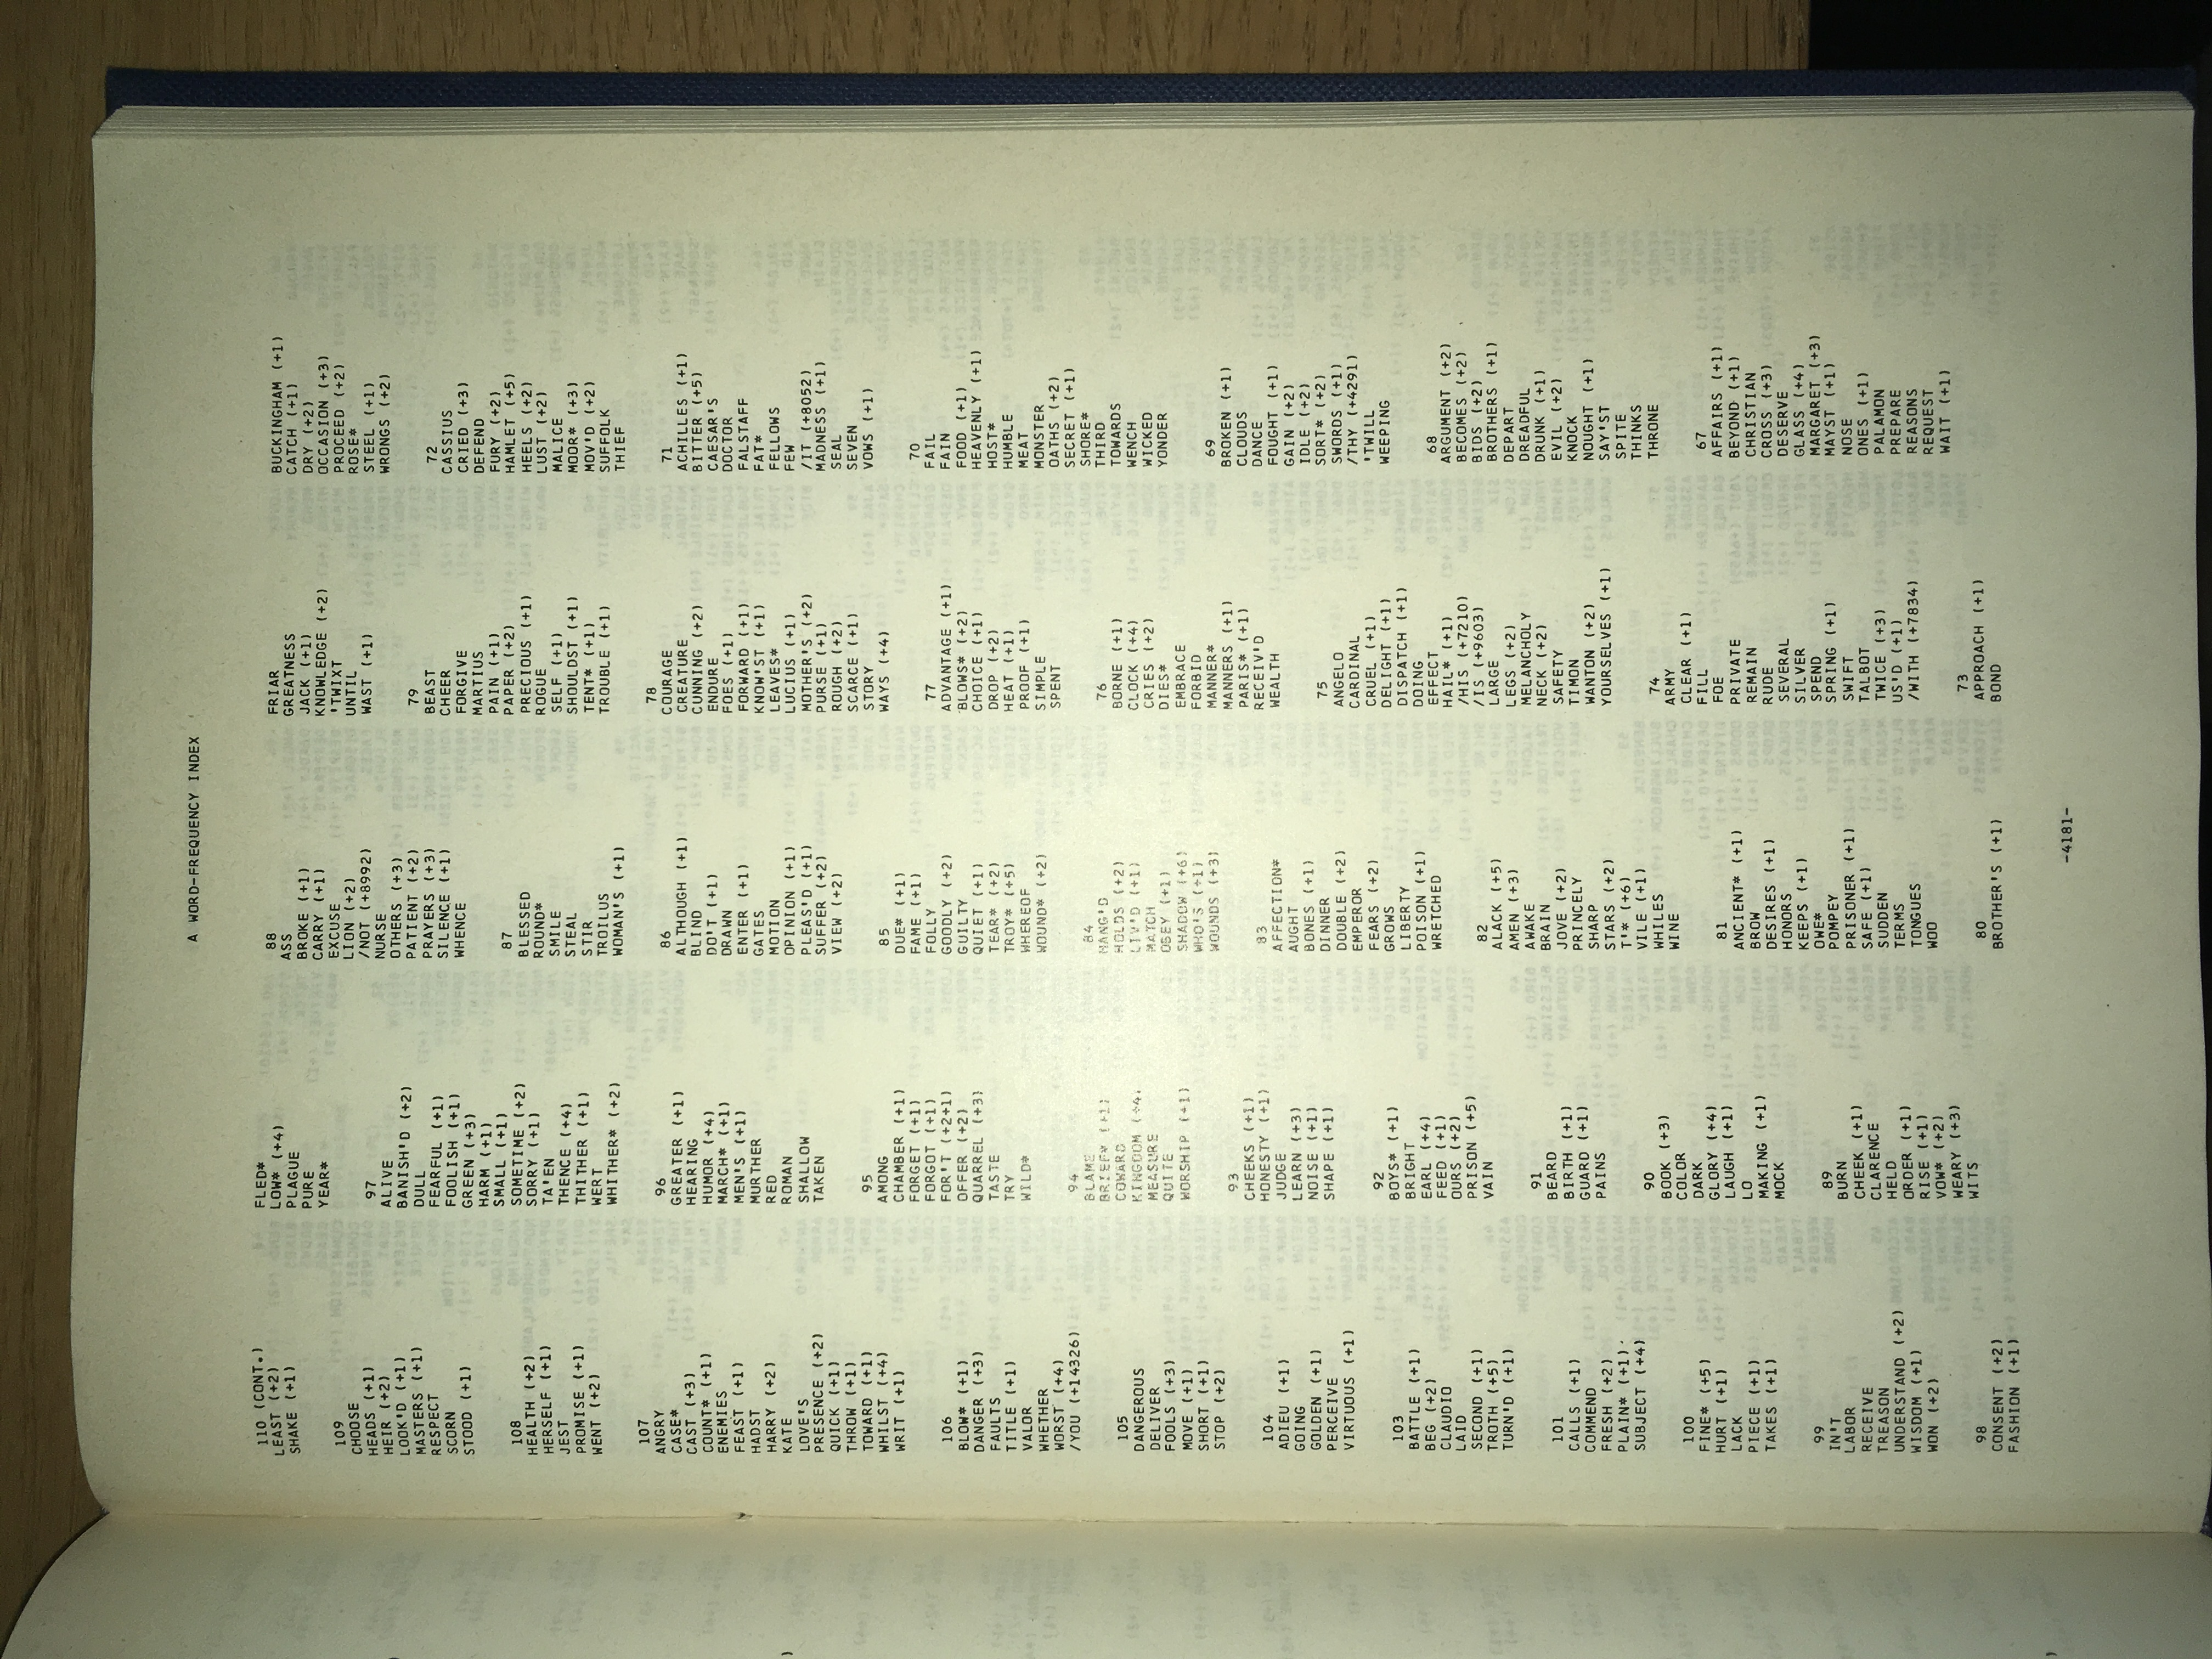
\includegraphics[width=3.25in,angle=270]{../compendium/Figures/IMG_4950.jpg}
	\caption{First page of Appendix~A in Volume~6 of \citet[p.~4177]{Spevack:1968qd}, showing very high frequency words (left), and typical page (p.~4181) showing words with frequencies 67 through 109 (right). }
	\label{fig:appendixa}
\end{figure}

Figure~\ref{fig:appendixadetail} shows detail from the right-hand display in Figure~\ref{fig:appendixa}, specifically the entries corresponding to the frequencies $x=99$ and $x=100$.  The number of words shown, $x_{99}=7$ and $x_{100}=5$ agree with the corresponding entries in Table~1 of ET.

\begin{figure}
	\centering
	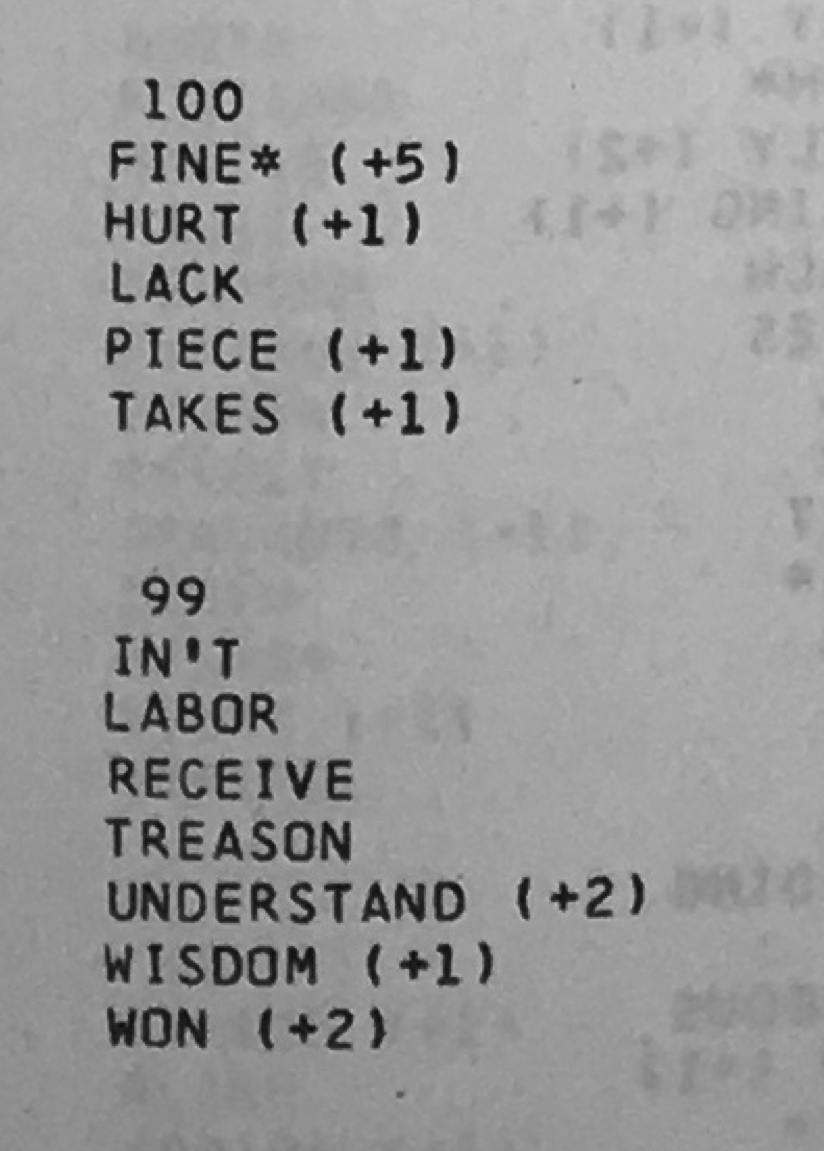
\includegraphics[height=2in]{../compendium/Figures/IMG_4950_detail.pdf}
	\caption[]{Detail from Appendix~A in Volume~6 of \citet[p.~4181]{Spevack:1968qd}, showing words that appear 99 and 100 times in Shakespeare. The asterisk appearing next to the word \texttt{FINE} indicates that the word is a homograph, that is a word type that Shakespeare used with at least two different meanings in different settings.  ``Fine,'' for instance, can be a noun indicating a penalty, a verb meaning to purify, or an adjective meaning exquisite, among many other meanings.  In any event, homographs have no affect on any of the analyses (or models) in ET.}
	\label{fig:appendixadetail}
\end{figure}

{\LARGE \color{red}\citeauthor{Efron:1976zs} report}
% subsection high_frequency_counts (end)

\subsection{Reproducing Table~1 of Efron and Thisted} % (fold)
\label{sub:et_table_1}
{\LARGE \color{red} TO WRITE UP}

% subsection et_table_1 (end)

\subsection{Double counting} % (fold)
\label{sub:double_counting}

Although Spevack reports that the most common word in Shakespeare (``the'') appears 27457 times, he also reports that it appears an additional 278 times in square brackets in the Evans edition of Shakespeare on which the Spevack \textit{Concordance} is based.  These words resulting from editorial emendation are counted as separate word types in the ET and Gani/Saunders compilation, and this is probably an error.  The bracketed words should be counted as if they were used by Shakespeare, as they constitute the best editorial asssessment of what Shakespeare wrote.  In that case, both $x_{27457}$ and $x_{278}$ are each too large by one, and $x_{27735}$ should be incremented by one).  In this case, the total number of unique words reported in ET is too large, as words that ever appear in editorial brackets are counted twice.

Figure~\ref{fig:appendixadetail} illustrates how the effect of double counting is potentially substantial. For instance, four of the five entries for $x=100$ have parenthetical counts that correspond to the number of times the same word appears in editorial brackets.  Thus, only one of the five words listed under $x=100$ appeared exactly 100 times!

An alternative way to account for bracketed words would be to say that, because they are a result of editorial rather than Shakespearean action, that they should be disregarded entirely.  In that case, $x_{27457}$ would remain at one, but $x_{278}$ should be decremented by one to account for disregarding ``[the]''.

In either case, the total number of word types reported by ET is be overstated.  Indeed, Spevack reports that the total number of unique words in the Shakespearean corpus is 29066 (Spevack, vol 4, p.~1), and this figure is echoed by Gani and Saunders. Both are at odds with the total of 31534 reported in ET.  This suggests that roughly 2500 words were counted twice.

Recalculating Table~3 and everything that follows from it to take this double counting into account would require a substantial amount of effort to identify, extract, and correct the myriad instances of this type of double counting, an effort which I may take on at a later point in time.

% subsection double_counting (end)
% section data_sources (end)


\section{Hardware and operating system environments} % (fold)
\label{sec:hardware_and_operating_system_environments}

The main calculations (for Table~~3, for instance) were carried out on a Wang 2200B, a high-end business-oriented microcomputer.  A dialect of BASIC, very close to the original language described by Kemeny and Kurtz, and Keller in 1964\footnote{In fact, the only available variable names were the single letters A--Z and a letter followed by a single digit.  Array names had the same limitation, but the array and scalar namespaces were distinct.   Thus, one could have both a scalar variable \texttt{W} and an array named \texttt{W}, leading to constructions like \texttt{MAT W=(1/W)*W}, a line that actually appears in the code used to generate Table~3.} was embedded in its microcode.  It could only be programmed in BASIC.  Programs had to be entered at the keyboard, but could be stored and retrieved using a cassette tape recorder. Programs could be stored for posterity (and future reproducibility studies), provided posterity was not expected to last longer than two or three years.
s
The programs written in PL/I (a general-purpose programming language of the day) and the ones written as input to MPS/360 were run on an IBM/360 mainframe computer.  The days of using punched cards for such programs were waning, and it had just become possible to create, save, and edit text files interactively, and then to submit them as if they were stacks of punched cards for execution.  I do not recall whether I carted boxes of punched computer cards with me when I left Stanford for Chicago in 1976, but I can say definitively that none remain.

One of the challenges for reproducible research is that programming languages and software systems (such as Stata, R, or MPS/360) can either become obsolete or evolve to the point of unrecognizability (and incompatibility).  The hardware on which programs run also becomes obsolete or unavailable.  And even were the same hardware still available, the underlying programs may no longer run under current versions of the hardware's operating system.

There is one additional aspect of computer hardware that can affect reproducibility, especially in the context of the Shakespeare example.  In 1975, numerics were poorly understood by computer architects of the day.  The first IEEE Standards for floating-point computation did not exist until 1985, ten years after our work.  As a result, the numerical quality of computed results could be quite poor, and without there being any indicator that that was the case.  So even if the calculations could be reproduced on the hardware of the day, there would still be good reason to check to see whether the results are different today!

% section hardware_and_operating_system_environments (end)

\section{Processes and choices} % (fold)
\label{sec:processes_and_choices}

Even if the data sources underlying the computations are verified and all of the software, hardware, and operating systems are available and can be used, reproducibility is not guaranteed.  The output of those programs, in our case, depended on initial values for parameters that we had to select and enter.  Without a record of which parameter values were used to obtain the results reported in the paper, and without mathematical guarantees that the results are insensitive to starting values, we cannot be certain as to how the results were actually obtained.  (This was a major motivation for \citet{Buckheit:1995hl}.)

% section processes_and_choices (end)


\chapter[]{A simple unbiased estimator}

The maximum likelihood estimates for the Fisher negative binomial model, which serves as a benchmark for many of the results in ET, are presented in Table~3.  They, and the calculations leading up to them, will be the focus for the rest of this paper.

The very first nontrivial calculation in ET is expression~(2.5), which provides a simple unbiased estimate for $\hat\Delta(1)$, the expected number of new words to be seen in a newly-discovered corpus of work equal in size to the corpus of Shakespeare that we already have in hand.  The expression reduces to
\begin{equation}
	\hat\Delta(1) = n_1-n_2+n_3-n_4+\ldots\;,
	\label{eq:unbiased}
\end{equation}
and expression~(2.5) asserts that $\hat\Delta(1)=11430$.

We report the first 100 values of $n_x$ in our Table~1. As it turns out, however, the alternating sum of those values turns out to be 11486, a figure that is about half a percent larger that the one reported in the paper!

What is going on?  One possibility is that we used fewer than the 100 values in Table~1 in calculating (\ref{eq:unbiased})  However, none of the partial sums
$$
s_m=\sum_{x=1}^m (-1)^{x+1} n_x$$
equals 11430.  

A second possibility is that we actually had \textit{all} of the $n_x$ values (up to $x=27457$)in hand and that we used them all to obtain our estimate.  However, if we append the frequency counts for $x>100$ to those in Table~1, expression (\ref{eq:unbiased}) turns out to be 11543.

A third possibility is that we calculated $\hat\Delta(1)$ using frequency counts from an early version of the dataset that contained errors, that we subsequently corrected the errors in Table~1, but we didn't recalculate $\hat\Delta(1)$.  In fact, I discovered a hand-written version of Table~1 in my files, and three of the counts in that version differ from the counts reported in Table~1 of ET.  The hand-written table is shown in Figure~\ref{fig:hand-Table1}.  The hand-written entries that differ are $n^*_6=887$ (instead of~837), $n^*_{94}=12$ (instead of~7), and $n^*_{97}=13$ (instead of~15).  When expression~(\ref{eq:unbiased}) is applied to the hand-written table, the resulting estimate is $\hat\Delta^*(1) = 11429$, almost---but not exactly---the value of 11430 reported in ET!

\begin{figure}
	\centering
	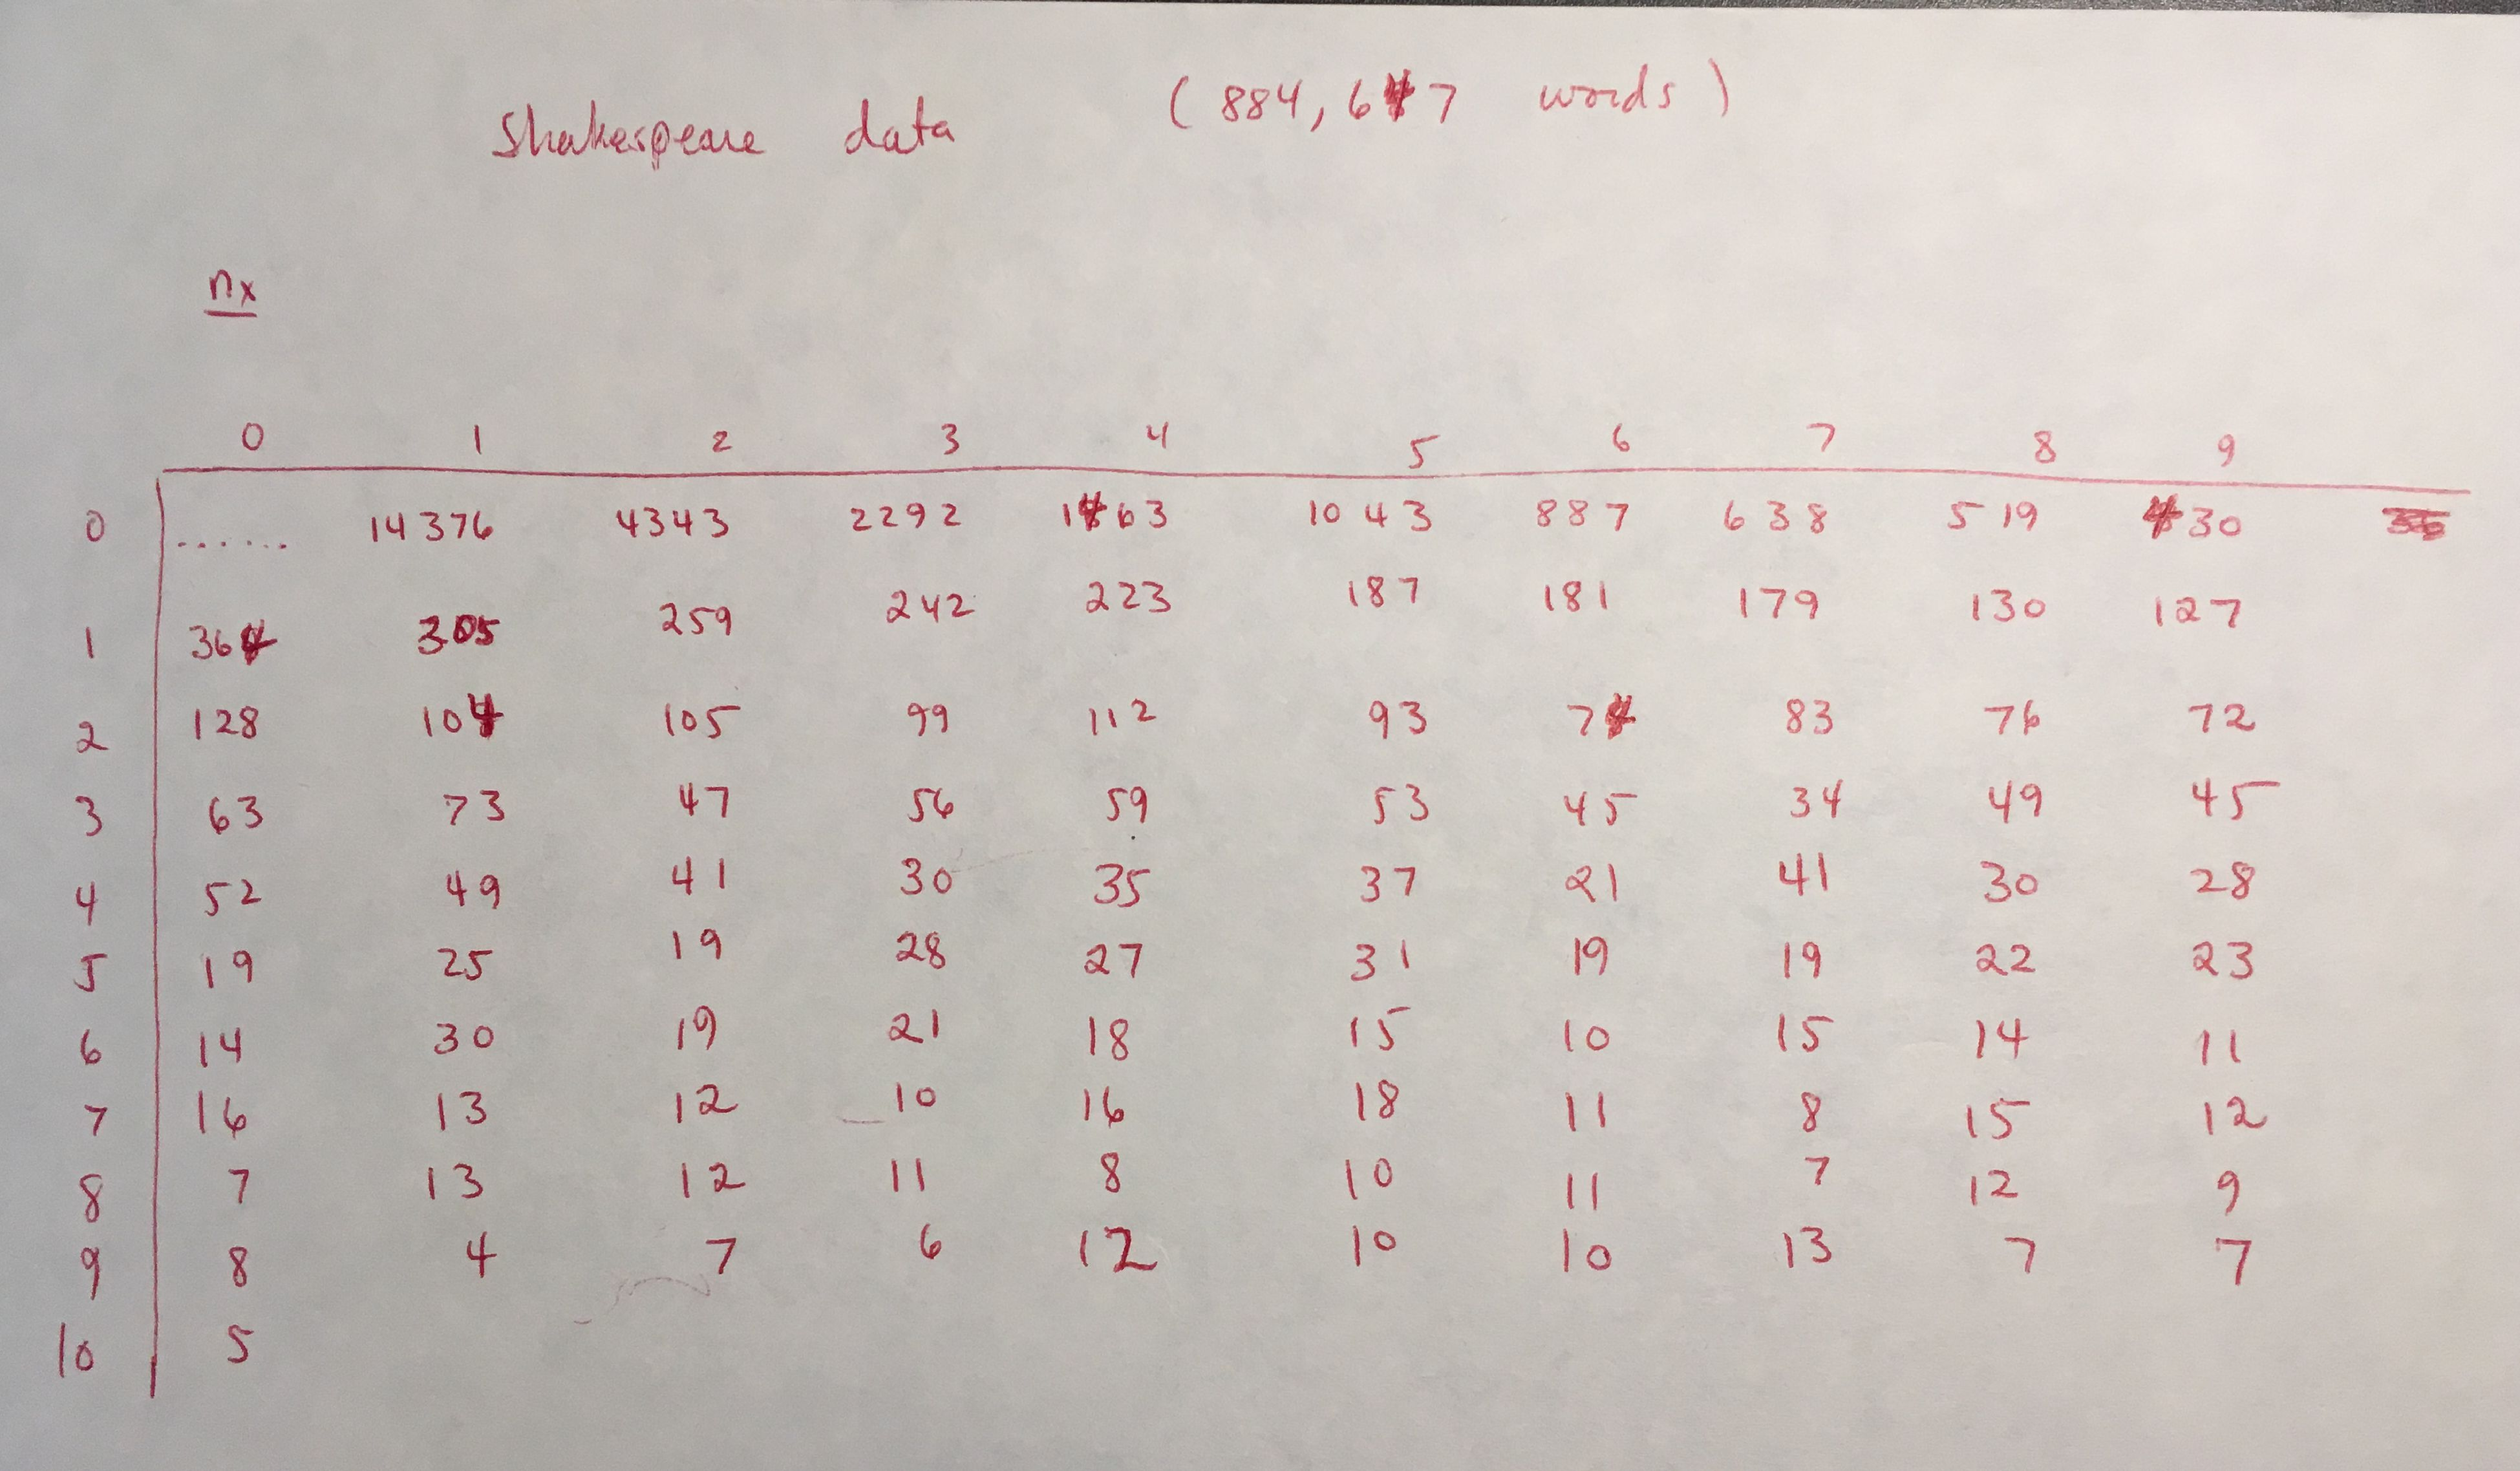
\includegraphics[width=5in]{Photos/Handwritten-table-1-version.pdf}
	\caption{Probably an early version of Table~1 from ET, which differs in three locations from the from the published text (at $x=6, 94, 97$).}
	\label{fig:hand-Table1}
\end{figure}

\begin{quotation}
	\textit{Lesson.}  Archive data sets and version control them, and run all scripts only on the final version.
\end{quotation}

A fourth possibility is that the calculation was done by hand using a calculator rather than computer program.  In that case, one or more frequencies could have been entered in error.  For instance, if $x_{33}=56$ were accidentally omitted from the calculation---an error easily done when doing the calculation by hand---then the end result for $\hat\Delta_{100}(1)$ would be exactly 11430.

A fifth possiblity also posits hand calculation.  The person doing the calculation could have lost track of the alternating sign parity at some point.  Specifically, if instead of subtracting $n_{38}$ from the running sum, $n_{38}$ were added instead, and then $n_{39}$ subtracted, $n_{40}$ added, and so forth, then the resulting calculation would again produce 11430 exactly.

Note, too, that as $x_0$ increases, the values of $\hat\Delta_x(1)$ oscillate (see Figure~\ref{fig:delta1hat}).  This suggests that a smoothed version, say the average of $\hat\Delta_{99}(1)$ and $\hat\Delta_{100}(1)$ would be superior.  So a fifth possibility is that we did some smoothing and forgot to mention it in the paper.

\begin{figure}
	\centering
	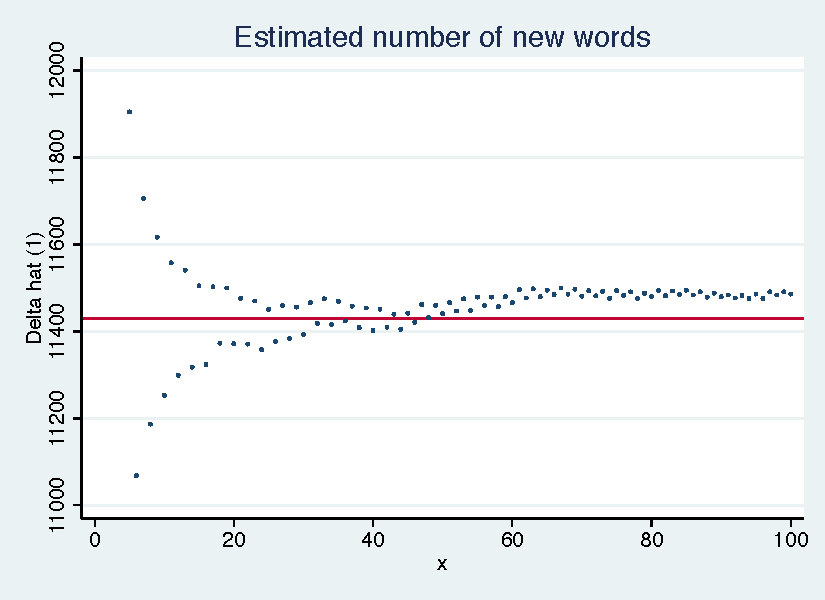
\includegraphics[width=3in]{../compendium/Figures/delta1hat.pdf}
	\caption{As $x$ increases, $\hat\Delta_x(1)$ oscillates.  The solid line is at $\hat\Delta(1)=11430$, the figure cited in the text of ET.  Values for $x<5$ are omitted to show detail.}
	\label{fig:delta1hat}
\end{figure}

In fact, the values for $\hat\Delta_x(1)$ for $x$ near $x_0=40$---a choice used repeatedly later in the paper---are reasonably close to 11430; the average of $\hat\Delta_{37}(1)$ and $\hat\Delta_{38}(1)$ is 11433.5, and the average of $\hat\Delta_{39}(1)$ and $\hat\Delta_{40}(1)$ is 11428.

In my view, the most likely explanation for the error in expression~(2.5) of ET is that it arose in the process of hand calculation, with a parity error being the simplest explanation.  The Stata script with the calculations carried out to support the explorations in this section is reproduced in Appendix~\ref{cha:simple_unbiased_estimate_for_delta_1}.

So in the end, if 11430 is actually an error and the correct number is 11486, what difference would it make to the rest of the ET paper?  The answer is not much, except that the Fisher negative binomial estimate that we report (using $x_0=40$) is 11483, virtually identical to the simple unbiased estimator based on $x_0=100$ alternating sums!

\chapter[]{The Fisher negative binomial model} % (fold)
\label{cha:the_fisher_negative_binomial_model}

So let's move on to the heart of ET, our study of a negative binomial model for species counts advanced by Fisher.  These are some notes that I wrote to the Chinese student whose query initiated this inquiry, pointing out some tips in dealing with the somewhat tricky maximum likelihood calculation.

The calculation is not, actually, a straightforward negative binomial problem.  Rather, the problem is to maximize a multinomial likelihood where the probabilities are proportional to the parameterized negative binomial.  (Equivalently, we are maximizing a conditional negative binomial likelihood, conditional on observing only $1 \le x \le x_0$).  Norming these probabilities to sum to one introduces the trickiness.


\medskip
\textbf{Notes on Efron and Thisted (1976)}

Ronald Thisted
\medskip

The maximum likelihood calculation is tricky.  Consider just the first row of Table~3, which only looks at the first five word types (those seen once, twice, up to five times). The likelihood is 

$$
L(p_1, p_2, \ldots, p_5) = p_1^{n_1}p_2^{n_2}p_3^{n_3}p_4^{n_4}p_5^{n_5}, \eqno(1)
$$
where
$$p_x = c{\Gamma(x+\alpha)\over x!\Gamma(1+\alpha)}\gamma^{x-1}, \eqno(2)$$
and where $c$ is the constant that makes $\sum_1^5 p_x=1$.
Maximizing the likelihood with respect to $\alpha$ and $\gamma$ is equivalent to maximizing the logarithm of the likelihood, which is considerably easy to work with.  Notice that $c^N$ can be factored out of the likelihood, so that the value of $c$ doesn't matter, so long as in the end the estimated probabilities add up to one.

The log likelihood then looks like this:
$$ \ell(p_1, p_2, \ldots, p_5) = \ell(\alpha, \gamma) = \sum_{x=1}^5 n_x \ln(p_x), \eqno(3)
$$           
where each $p_x$ is written in terms of $\alpha$ and $\gamma$.  Since
$$ p_x = \left(x+\alpha \over x+1\right)\gamma \cdot p_{x-1}, \eqno(4)$$
for any given values for $\alpha$ and $\gamma$, one can take $p_1=1$, calculate $p_2$ through $p_5$ using the recursion stated above, calculate $c=\sum p_x$, and then divide each of the $p_x$ values by $c$ to make them sum to one (as they are probabilities).
With the $p_x$ values corresponding to $\alpha$ and $\gamma$, the next step is to calculate the log likelihood.

One approach to finding the maximum likelihood estimates for $\alpha$ and $\gamma$ is by iterative search.  Select starting values such as $\alpha=0$ and $\gamma=1$ for the two parameters.  Without changing $\gamma$, calculate the log likelihood for different choices of $\alpha$.  When the log likelihood stops increasing, take smaller steps within the interval containing the maximum until you get adequate precision.  Then fix $\alpha$ at this new value and then proceed to do the same thing with $\gamma$.  When this step converges, hold $\gamma$ at its new value and repeat the process with $\alpha$.  Alternate between the two parameters until you have adequate precision. 

Unfortunately, this process converges very slowly to the maximum value, in part because the likelihood function is very flat near the maximum.

Other approaches, such as Fisher scoring or Newton-Raphson, can optimize for both $\alpha$ and $\gamma$ at the same time, but they require derivatives of the log likelihood function.  There are also methods that numerically approximate the derivatives.  I believe that the ``Solver'' functions in Microsoft Excel use that approach.

Here is an approach to doing the calculations of the log-likelihood in Excel. First, create two cells that hold $\alpha$ and $\gamma$, (a) a column with $x$ values (1 through 5, or 40), (b) a column of $n_x$ values, (c) a column with values proportional to equation~(2), calculated using the recursion of equation~(4), a cell that sums the entries in that column, (d) a column that divides column (c) by the sum--these are the estimated probabilities $\hat p_x$, (e) a column with that row's contribution to the log likelihood ($n_x \ln(\hat p_x)$), and then the sum of column~(e), which gives the log-likelihood.  By changing the values for $\alpha$ and $\gamma$, the log likelihood is automatically updated.

There is an {R} package, \texttt{https://r-how.com/packages/preseqR}, that may do some (or all) of the negative binomial fitting to data such as these, although I haven't tried it.

% chapter the_fisher_negative_binomial_model (end)

\chapter{Notes on additional computations} % (fold)
\label{cha:notes_on_additional_computations}

	Discussion of issues related to Tables~4 thorugh~6, especially the linear programming software issue.
	
% chapter notes_on_additional_computations (end)

\newpage
\appendix

\chapter{BASIC MLE program} % (fold)
\label{cha:basic_mle_program}
{\footnotesize\parindent=0pt \obeylines \texttt{\input{../compendium/Programs/mle.bas.txt}}
\parindent=1em
% chapter basic_mle_program (end)

\newpage
\chapter{Stata negative binomial log likelihood} % (fold)
\label{cha:stata_negative_binomial_log_likelihood}
{\footnotesize\parindent=0pt \obeylines\obeyspaces \texttt{\verbatiminput{../compendium/Analysis/et.do}}
% chapter stata_negative_binomial_log_likelihood (end)

\newpage
\chapter{Stata Table 3 reproduction} % (fold)
\label{cha:stata_table_3_reproduction}
{\footnotesize\parindent=0pt \obeylines\obeyspaces \texttt{\verbatiminput{../compendium/Analysis/table3mlFromTable1.do}}
% chapter stata_table_3_reproduction (end)

\newpage
\chapter{Example of Stata \texttt{ml} output} % (fold)
\label{cha:stata_example}
% Example showing standard errors and auxiliary calculations from Stata for x_0=40

\parindent=1em

Stata's \texttt{ml} command is a general-purpose optimizer that is designed to provide standard inferential tools in a standardized format as a by-product.  The program scripts \texttt{et.do} and \texttt{et1.do} provide the code needed to calculate the log likelihood for the conditional negative binomial model considered in Section~3 of \citet{Efron:1976zs}, the former parameterized using $\beta$ and the latter parameterized using $\gamma$.

The tables in section~\ref{sec:computer_programs} were produced by a script that suppressed the standard output from each individual estimation command, instead compiling and printing only the tabular results corresponding to Table~3 of \citeauthor{Efron:1976zs}.  To illustrate the utility of the approach using Stata, the output below shows estimates of $\alpha$, $\beta$, and $\gamma$, together with their standard errors and confidence intervals.

Here are the results for $x_0=40$, the setting used for several purposes in ET.  Lines that start with a period show inputs to Stata.  In this example we explicitly provide initial values to the \texttt{ml} maximizer, but using Stata's defaults produce virtually the same result, differing only by one unit in the sixth decimal place of $\hat\alpha$.  The estimate for $\alpha$ is $\hat\alpha=-0.3973$, and its standard error is $0.006$.  The two estimates are associated in the output below with \texttt{eq1:\_cons} ($\alpha$) and \texttt{eq2:\_cons} ($\beta$).

{\obeylines\obeyspaces
\begin{verbatim}
. ml model d0 et (nx=) () in 1/40
. ml init eq1:_cons=-0.4 eq2:_cons=50
. ml maximize, nolog

                                                Number of obs     =         40
                                                Wald chi2(0)      =          .
Log likelihood = -61615.249                     Prob > chi2       =          .

------------------------------------------------------------------------------
          nx |      Coef.   Std. Err.      z    P>|z|     [95% Conf. Interval]
-------------+----------------------------------------------------------------
eq1          |
       _cons |  -.3973074   .0059839   -66.40   0.000    -.4090355   -.3855792
-------------+----------------------------------------------------------------
eq2          |
       _cons |   112.2214   18.51752     6.06   0.000     75.92778    148.5151
------------------------------------------------------------------------------

. scalar gamma = _b[#2:_cons]/(1+_b[#2:_cons])
. display "Delta-hat_ml(1)= " %8.0f -nx[1]*((1+gamma)^(-_b[_cons]) -1)/(_b[_cons]*gamma) "  Gamma= " %7.5f gamma
Delta-hat_ml(1)=    11490  Gamma= 0.99117

. // get standard error for gamma hat and for Delta-hat(1)
. nlcom _b[#2:_cons]/(1+_b[#2:_cons])

       _nl_1:  _b[#2:_cons]/(1+_b[#2:_cons])

------------------------------------------------------------------------------
          nx |      Coef.   Std. Err.      z    P>|z|     [95% Conf. Interval]
-------------+----------------------------------------------------------------
       _nl_1 |   .9911678   .0014445   686.15   0.000     .9883365     .993999
------------------------------------------------------------------------------
\end{verbatim}
\newpage
Usefully, Stata can not only calculate $\hat\Delta(1)$, but can also obtain its standard error via the delta method.

\begin{verbatim}
. nlcom -nx[1]*((1+gamma)^(-_b[_cons]) -1)/(_b[_cons]*gamma)

       _nl_1:  -nx[1]*((1+gamma)^(-_b[_cons]) -1)/(_b[_cons]*gamma)

------------------------------------------------------------------------------
          nx |      Coef.   Std. Err.      z    P>|z|     [95% Conf. Interval]
-------------+----------------------------------------------------------------
       _nl_1 |   11489.66   24.75408   464.15   0.000     11441.15    11538.18
------------------------------------------------------------------------------
\end{verbatim}
}

By repeating the calculation parameterizing using $\gamma$ ($=\beta/(1+\beta)$) instead of $\beta$, we obtain standard errors for $\hat\gamma$ as well.  Note that the log likelihood is the same for both parametrizatoins.  Because $\gamma$ is constrained to be strictly less than one (by its relationship to $\beta$), and because our estimates for $\gamma$ are near that upper boundary, we would expect the computation based on $\beta$ (which is unconstrained) to be somewhat more stable numerically, and for that reason our computations in the text are based on the $\beta$ parameterization.

\begin{verbatim}
. // repeat using gamma parameterization
. ml model d0 et1 (nx=) () in 1/40

. ml maximize, nolog
initial:       log likelihood =     -<inf>  (could not be evaluated)
feasible:      log likelihood = -96277.713
rescale:       log likelihood = -96277.713
rescale eq:    log likelihood = -85253.513

                                                Number of obs     =         40
                                                Wald chi2(0)      =          .
Log likelihood = -61615.249                     Prob > chi2       =          .

------------------------------------------------------------------------------
          nx |      Coef.   Std. Err.      z    P>|z|     [95% Conf. Interval]
-------------+----------------------------------------------------------------
eq1          |
       _cons |   -.397306   .0059838   -66.40   0.000     -.409034   -.3855779
-------------+----------------------------------------------------------------
eq2          |
       _cons |   .9911673   .0014445   686.15   0.000     .9883361    .9939986
------------------------------------------------------------------------------
\end{verbatim}
% chapter stata_example (end)

\newpage
\chapter{Simple unbiased estimate for $\Delta(1)$} % (fold)
\label{cha:simple_unbiased_estimate_for_delta_1}
{\footnotesize\parindent=0pt \obeylines\obeyspaces \texttt{\verbatiminput{../compendium/Analysis/Equation2.5.do}}
% chapter simple_unbiased_estimate_for_delta_1 (end)

% \part{Memoir Supported Part I}
% \chapter[Chapter 1 TOC entry][Chapter One Heading]{Chapter One}
% \lipsum[1-13]
% \chapter{Chapter Two}
% \lipsum[1-14]
% \part{Memoir Supported Part II}
% \chapter{Another Part, Another Chapter}
% \lipsum[1-14]
% \appendix
% \part{Appendices go here}
% \chapter{Appendix I am}
% \lipsum[1-9]
% \chapter{Because I am appended}
% \lipsum[1-11]

\backmatter

% Bibliography goes here
% ----------------------

\bibliographystyle{plainnat}
\bibliography{../References/Efron80}

\end{document}
